\documentclass[11pt, oneside]{article} 
\usepackage{geometry}
\geometry{letterpaper} 
\usepackage{graphicx}
	
\usepackage{amssymb}
\usepackage{amsmath}
\usepackage{parskip}
\usepackage{color}
\usepackage{hyperref}

\graphicspath{{/Users/telliott_admin/Tex/png/}}
% \begin{center} 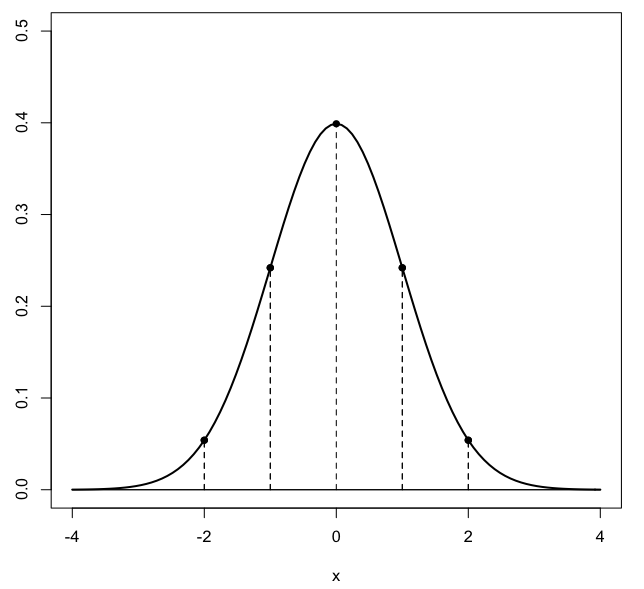
\includegraphics [scale=0.4] {gauss3.png} \end{center}

\title{Exponential to logarithm}
\date{}

\begin{document}
\maketitle
\Large

\label{sec:Exponential_to_logarithm}

The logarithm and the exponential function are inverses of each other.  We will prove this assertion here.

It seems reasonable enough if we plot them together.  The upper curve is $y = e^x$ and the lower one is $y = \ln x$.
\begin{center} 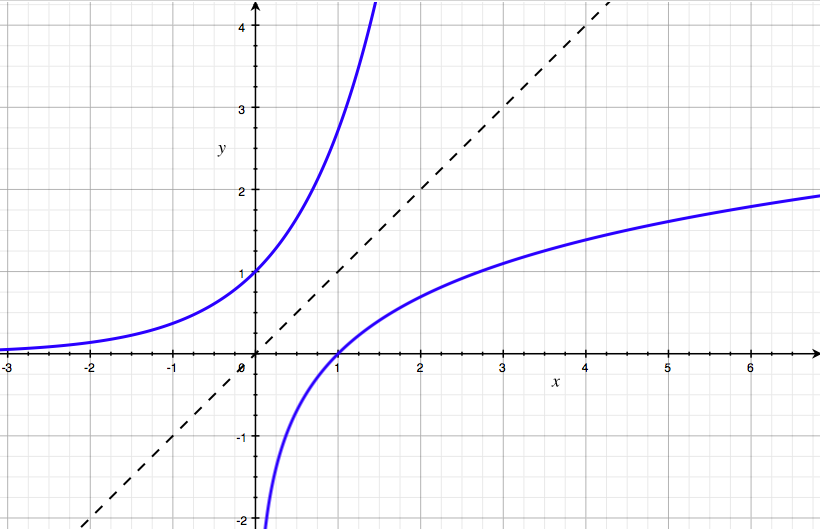
\includegraphics [scale=0.35] {log2.png} \end{center}

As inverse functions, $e^x$ and $\ln x$ are symmetric about the line $y=x$.

If we consider a particular $x$ value, for example $x=1$, then the slope of the curve $y=e^x = e$ at the point $(1,e)$ is the inverse of the slope of the curve $y= \ln x$ when $x=e$ (at the point $(e,1)$).

\subsection*{from exponential to logarithm}
The logarithm can be defined as follows:
\[ \int \frac{1}{t} \ dt = \ln(t) \]

It is possible to prove this starting from the assumption that $e$ is its own derivative, or that $e$ is the limit we discussed above.  Alternatively, we can start from this statement and derive the facts about $e$.  We will do the latter in a later chapter.

Now, differentiate both sides to find the derivative of the logarithm.  By the FTC:
\[ \frac{d}{dt} \int \frac{1}{t} \ dt  = \frac{1}{t}  = \frac{d}{dt} \ln(t) \]
This is great because we never did generate $x^{-1}$ by differentiating powers of $x$.  

And now we know how to go back the other way, using the definition that the exponential function is its own derivative to establish the first statement above.

The proof is so simple that if you blink, you'll miss it.
\[ y = e^x \]
\[ \frac{dy}{dx} = e^x = y \]
Invert
\[ \frac{dx}{dy} = \frac{1}{y} \]
\[ dx = \frac{1}{y} \ dy \]
Integrate
\[ \int dx = x = \int \frac{1}{y} \ dy \]
And what is $x$?  It is $\ln y$!
\[ \ln(y) = \int \frac{1}{y} \ dy \]
And since $y$ is just a letter, we can write the same for $x$, or $t$
\[ \ln x = \int \frac{1}{x} \ dx, \ \ \ \  \ln t = \int \frac{1}{t} \ dt \]
One of the prettiest things I've ever seen.

The math purists don't like it, but in general it is OK to do algebra with differentials.  One important restriction is that $dy/dx$ (and $dx/dy$) should not be equal to zero.  And a second one is that we just remember we are never passing to the limit, just getting really, really, really close.  (As close as you like).

Now that we have this definition, we have another way of estimating the value of $e$.  We add up the areas for little slices under the function $y=1/x$ until the total reaches $1$.  The corresponding value of $x=e$.
\begin{center}
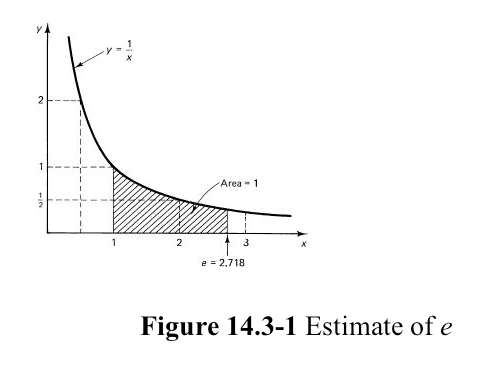
\includegraphics [scale=0.6] {log3.png}
\end{center}
(from Hamming).

For example, we might try intervals of $0.1$ and do
\[ 0.1 \cdot \frac{1}{1} + 0.1 \cdot \frac{1}{1.1} + 0.1 \cdot \frac{1}{1.2} + \dots + 0.1 \cdot \frac{1}{2.7} \]

\subsection*{reverse direction}
Above we showed that $(e^x)' = e^x$ implies
\[ \ln x = \int \frac{1}{x} \ dx \]
Differentiate both sides
\[ {\frac{d}{dx} \ln(x) = \frac{1}{x} } \]
We want to go backward now, to show that the derivative of the function $f(x) = e^x$ is itself.

Start with
\[ \ln(e^x) = x \]
\[ \frac{d}{dx} \ln(e^x) = \frac{d}{dx} x = 1 \]
but using the property we just proved and the chain rule, this is also
\[ \frac{d}{dx} \ln(e^x) = \frac{1}{e^x} \ \frac{d}{dx} e^x  \]
so these two expressions are equal and
\[ \frac{1}{e^x} \ \frac{d}{dx} e^x = 1  \] 
\[ \frac{d}{dx} e^x = e^x \]

Magic.

This is really the primordial differential equation.

\subsection*{Strang's view of the series}

Gil Strang has a nice introduction to the exponential (for real numbers).  He says we want to "construct a function" for $y = e^x$.  The first, amazing, property ($I$) is that the derivative of the function is equal to the function itself.
\[ y = y' \]

The second property, a boundary condition, is that at $x = 0$, we want $y = 1$.  That's because $e$ is not a variable and we want $e^x = e^0$ to be equal to $1$ like every other exponential we know.  [ A third property that will turn out to be true is $e^{x_1 + x_2} = e^{x_1} \cdot e^{x_2}$. ]

Using the second condition we write:
\[ y(x) = 1 \]

Whatever else is true, if there are no terms containing $x$ (because $x=0$) then $y = 1$.  By $I$ we must have that the derivative is equal to the function:
\[ y(x) = 1 \]
\[ y'(x) = 1 \]
But now, if we try to evaluate the derivative starting from $y(x)$, where does that $1$ come from?  It must come from
\[ y(x) = 1 + x \]
\[ y'(x) = 1 \]

Now, though, it's no longer true that $y = y'$ so we fix that
\[ y(x) = 1 + x \]
\[ y'(x) = 1 + x \]
And where does that $x$ come from in the derivative?  It must come from
\[ y(x) = 1 + x + \frac{x^2}{2} \]
\[ y'(x) = 1 + x \]

And so on ...  Following this procedure, we build up the definition
\[ y(x) = 1 + x + \frac{x^2}{2} + \frac{x^3}{3!} + \frac{x^4}{4!} + \dots  \]
\[ = \sum_0^{\infty} \frac{x^n}{n!} \]

The test for convergence of this infinite series is to find the values of $x$ such that:
\[ \lim_{n \rightarrow \infty} \frac{|A_{n+1}|}{|A_n|} < 1 \]
That is, we need
\[ \lim_{n \rightarrow \infty} \frac{x}{n+1} < 1  \]
But this is true for any $x$.


\end{document}  